%*****************************************************************************************
%*********************************** Sixth Chapter **************************************
%*****************************************************************************************

\chapter{Perovskite-coated metal islands}

\graphicspath{{Chapter6/Figures/}}

Interactions between localised surface plasmons (LSPs) and material in their environment can be used for a host of applications. For example sensitivity of the resonance frequency to the local dielectric function can be exploited in sensing devices \cite{Jensen2000, Xu2004, Malinsky2001, Royer1987}, while the large field enhancement caused by electron oscillations can be used to increase Raman signals \cite{Cade2009, Olson2001, Talley2005} or emission \cite{Toftegaard2011, Cho2010, Reboud2013, Blanco2004}. LSP resonances of noble metal nanoparticles can be tuned across the visible spectrum via their geometries, so fabrication of metal island nanostructures should be tuned to their application.

In this Chapter I will describe the creation of Au/Ag nano-islands overcoated with a perovskite layer, then use structural and optical characterisation techniques to explore how excitons are affected by electrons oscillations in the metal.

\section{Metal island films}
The morphology of a thin film depends on interactions between the film and substrate atoms (i.\,e.\,the diffusion of metal atoms on substrate surface), as well as external conditions such as deposition rate, substrate temperature and subsequent annealing steps \cite{Kaiser2002}. Deposition via evaporation is a heterogeneous nucleation process, and requires high vapour pressure. Various growth modes are possible, but for noble metal films deposited on glass the metal-metal interaction is stronger than the metal-substrate interaction, causing island formation on the substrate. With increased deposition time such islands can coalesce, either preserving the grain boundaries or forming a continuous structure.

Such metal island films (MIFs) are essentially nanoparticle arrays: if the islands are well separated (separation $l \gtrsim\,	$island diameter $d$) then there is no optical coupling between the particle resonances and we expect to see a single LSP resonance in optical spectra. The resonance wavelength of such arrays depend on the island geometry, and can be controlled by the deposited film thickness \cite{Walter2006, Sennett1950, Gupta2002, Gadenne2002, Lee1992}. As with nanoparticles we can model these islands as dipoles embedded in a medium with dielectric function $\epsilon$ to predict the resonance wavelength \cite{Yamaguchi1960, Yamaguchi1972, Yamaguchi1973, Doremus1966}.

\subsection{Experimental methods}
Glass substrates are prepared as described in Sec.\,\ref{sec:glass}. Metal deposition is performed using an Edwards resistance evaporator, under pressure $\sim4\times10^{-6}$\,mbar with deposition rate $\sim0.5$\,\AA/s. The substrates are not heated, and the deposited film thickness $t$ is determined by a 6\,MHz quartz crystal microbalance. To avoid oxidation, Ag samples are placed in a nitrogen purge dessication cabinet within 15\,minutes of fabrication, and only removed for further processing/characterisation. Annealed Au and Ag films are made by heating the samples at $200^{\circ}$C for 24\,hours. In order to create the CHPI overcoating, a CHPI/THF solution is spin coated onto the nanostructured films under a dehydrated atmosphere (layer thickness $\sim100$\,nm). The samples are then characterised using AFM, SEM, and white light microscopy. 400 unpolarised reflection ($R$) and transmission ($T$) spectra are taken over an area 0.5$\times$0.5mm$^{2}$, and due to sample uniformity, all 400 spectra are averaged to produce the data shown, where extinction is defined as $E=1-R-T$.

\subsection{Au metal island films}
\begin{figure}[h!] 
\centering    
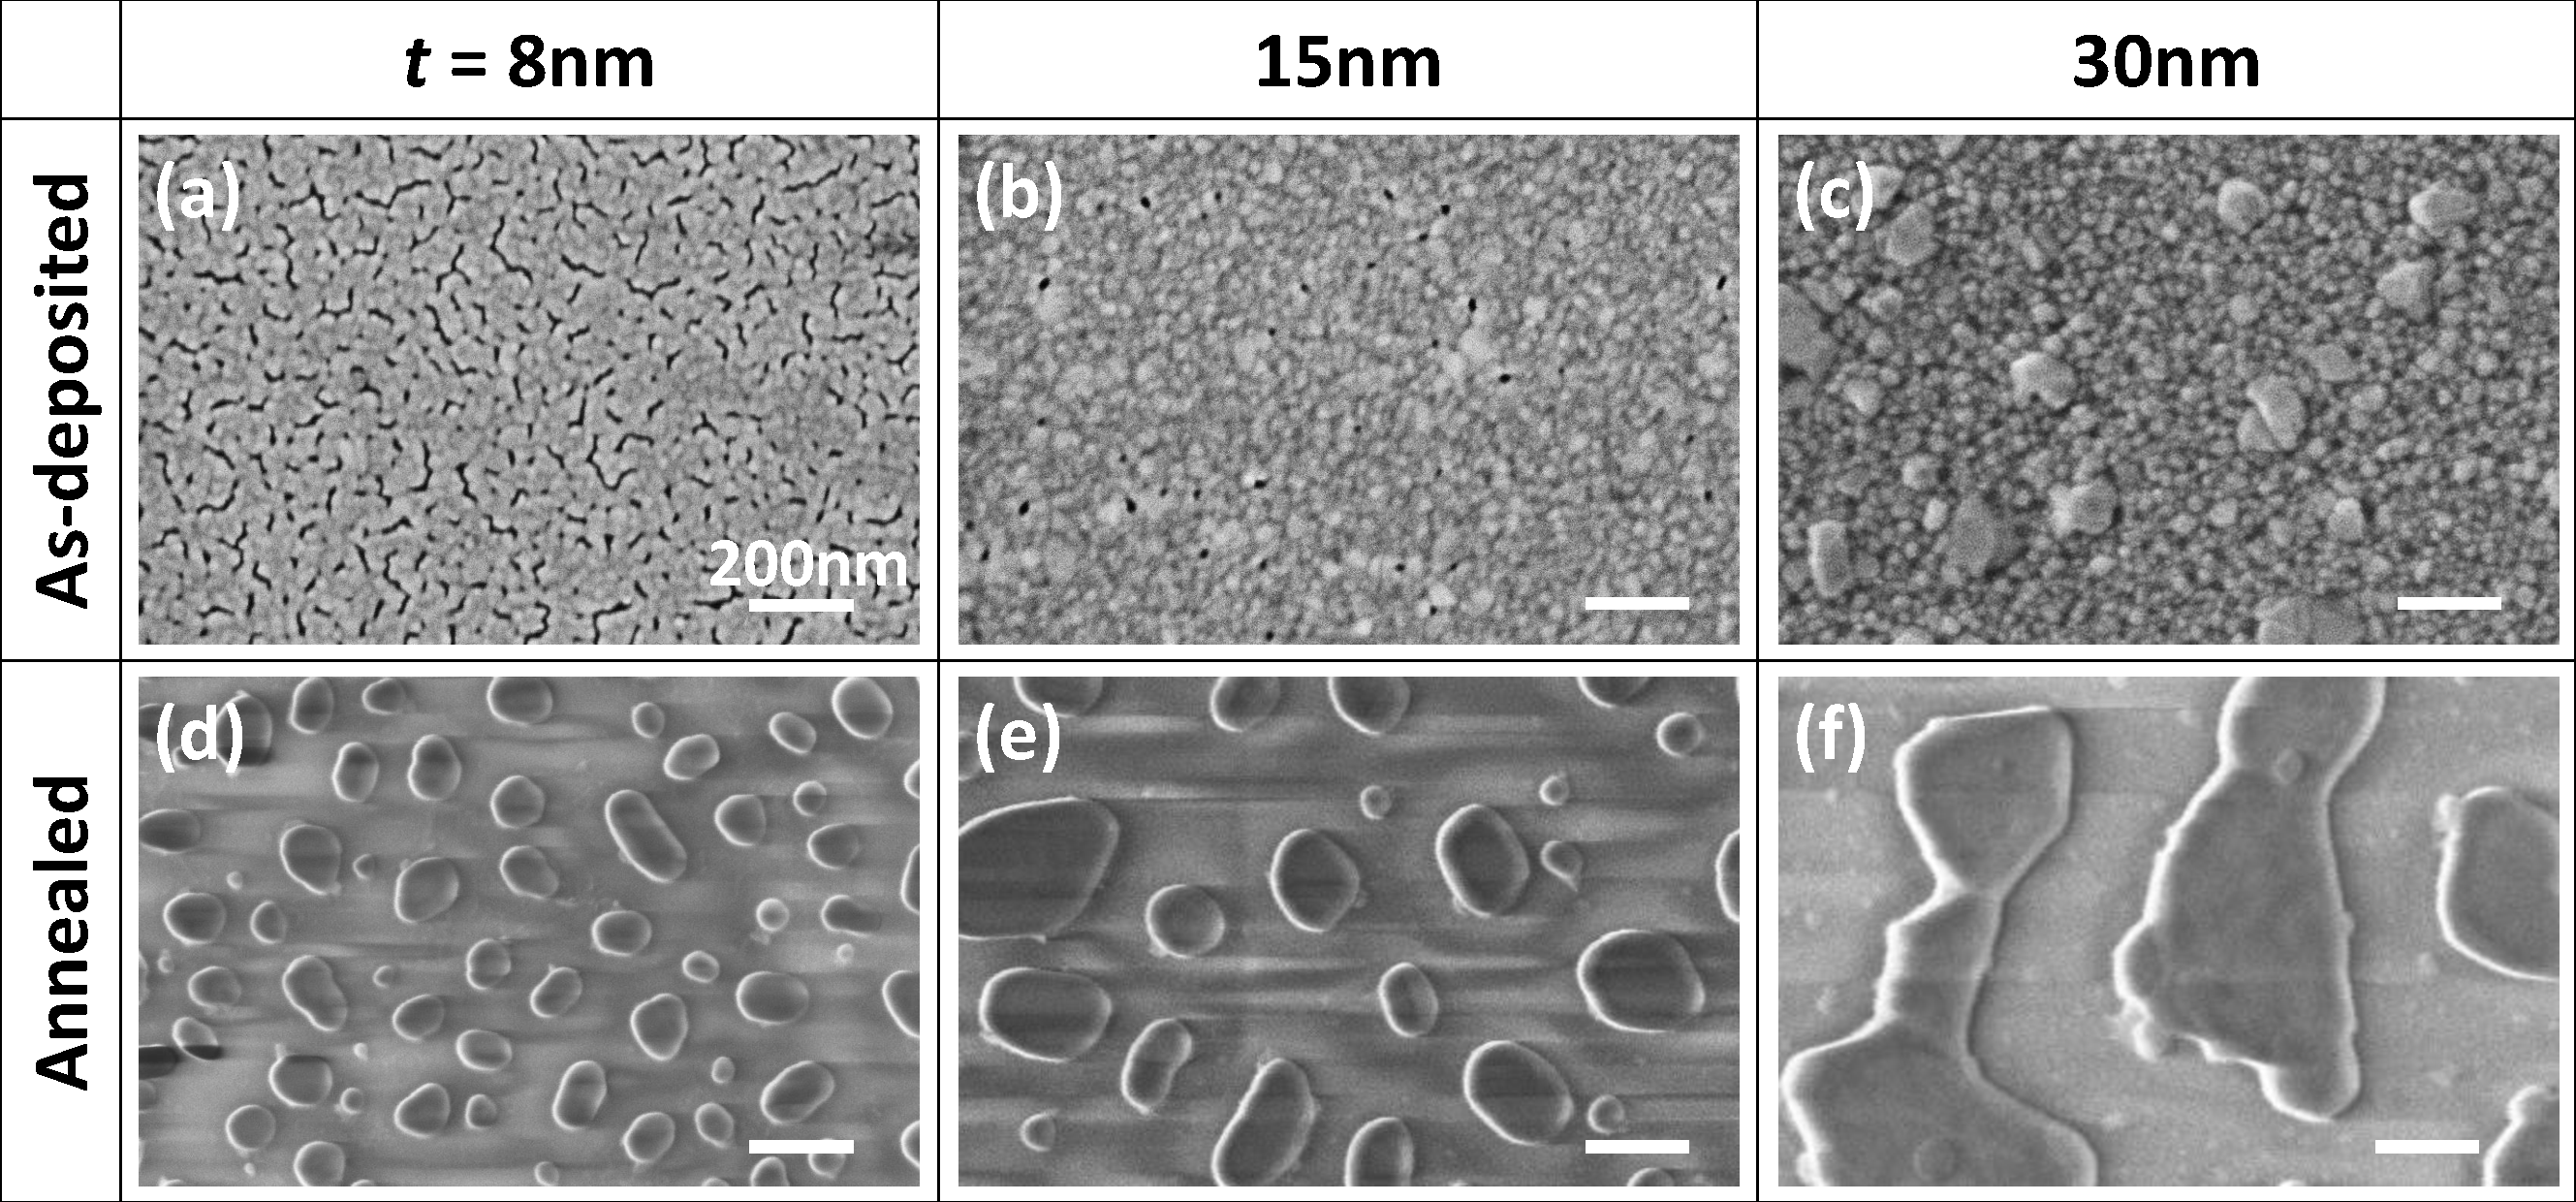
\includegraphics[width=\textwidth]{Fig1}
\caption{SEM images of (a-c) as-deposited and (d-f) annealed evaporated Au metal island films. The initial deposited film thickness $t$ is labelled.}
\label{6Fig1}
\end{figure}
SEM images of evaporated Au films on glass show the formation of a rough, non-uniform, but continuous film for $t=30$\,nm [Fig.\,\ref{6Fig1}(c)]. As $t$ decreases dewetting is observed as a result of weak Au-glass interactions [Figs.\,\ref{6Fig1}(a,b)]. During annealing, Au atoms diffuse and form distinct islands [Figs.\,\ref{6Fig1}(d-f)]. With decreasing $t$ the islands become more closely spaced and ellipsoidal, smaller in both lateral size $d$ and height $h$ [Fig.\,\ref{6Fig2}]. For $t=8$\,nm we observe islands with $4 \sim 50-100$\,nm, $h\sim$70\,nm, and $l \sim 100-200$\,nm. The decrease in size can also be seen optically in 100$\times$ magnification DF images, where scattering from the islands due to LSPs is broadband for $t=30$\,nm, but becomes progressively redder as the island size decreases [Fig.\,\ref{6Fig2}]. 
\begin{figure}[h!] 
\centering    
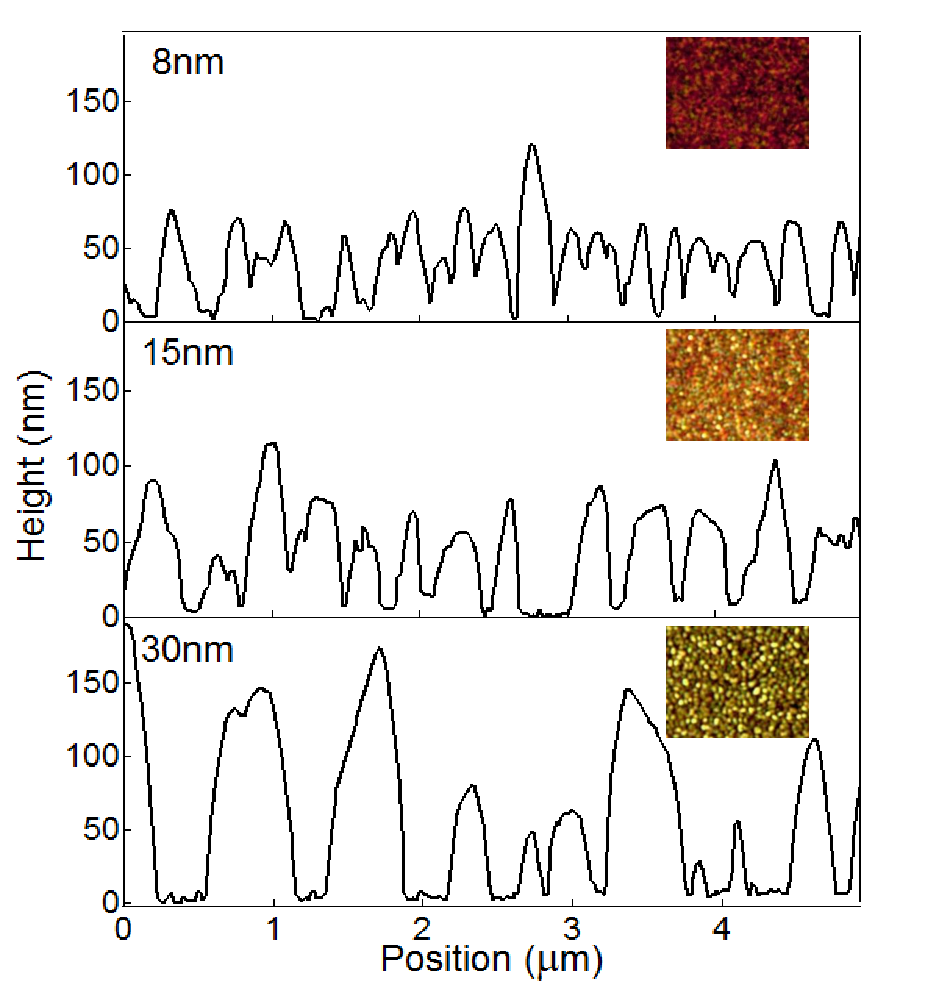
\includegraphics[width=0.8\textwidth]{Fig2}
\caption{AFM profiles of annealed Au metal island films. The deposited film thickness $t$ is labelled. Insets show 100$\times$ magnification DF images of the samples.}
\label{6Fig2}
\end{figure}

Fig.\,\ref{6Fig3} shows the extinction spectra for $t=8$\,nm as-deposited and annealed Au MIFs. We observe a resonance at 570\,nm in the extinction of the as-deposited film, however this is due to grains and therefore has a large linewidth of 245\,nm. In the annealed film we observe a resonance at 550\,nm with linewith 50\,nm due to island LSPs.

\subsection{CHPI-coated Au metal island films}
\begin{figure}[h!] 
\centering    
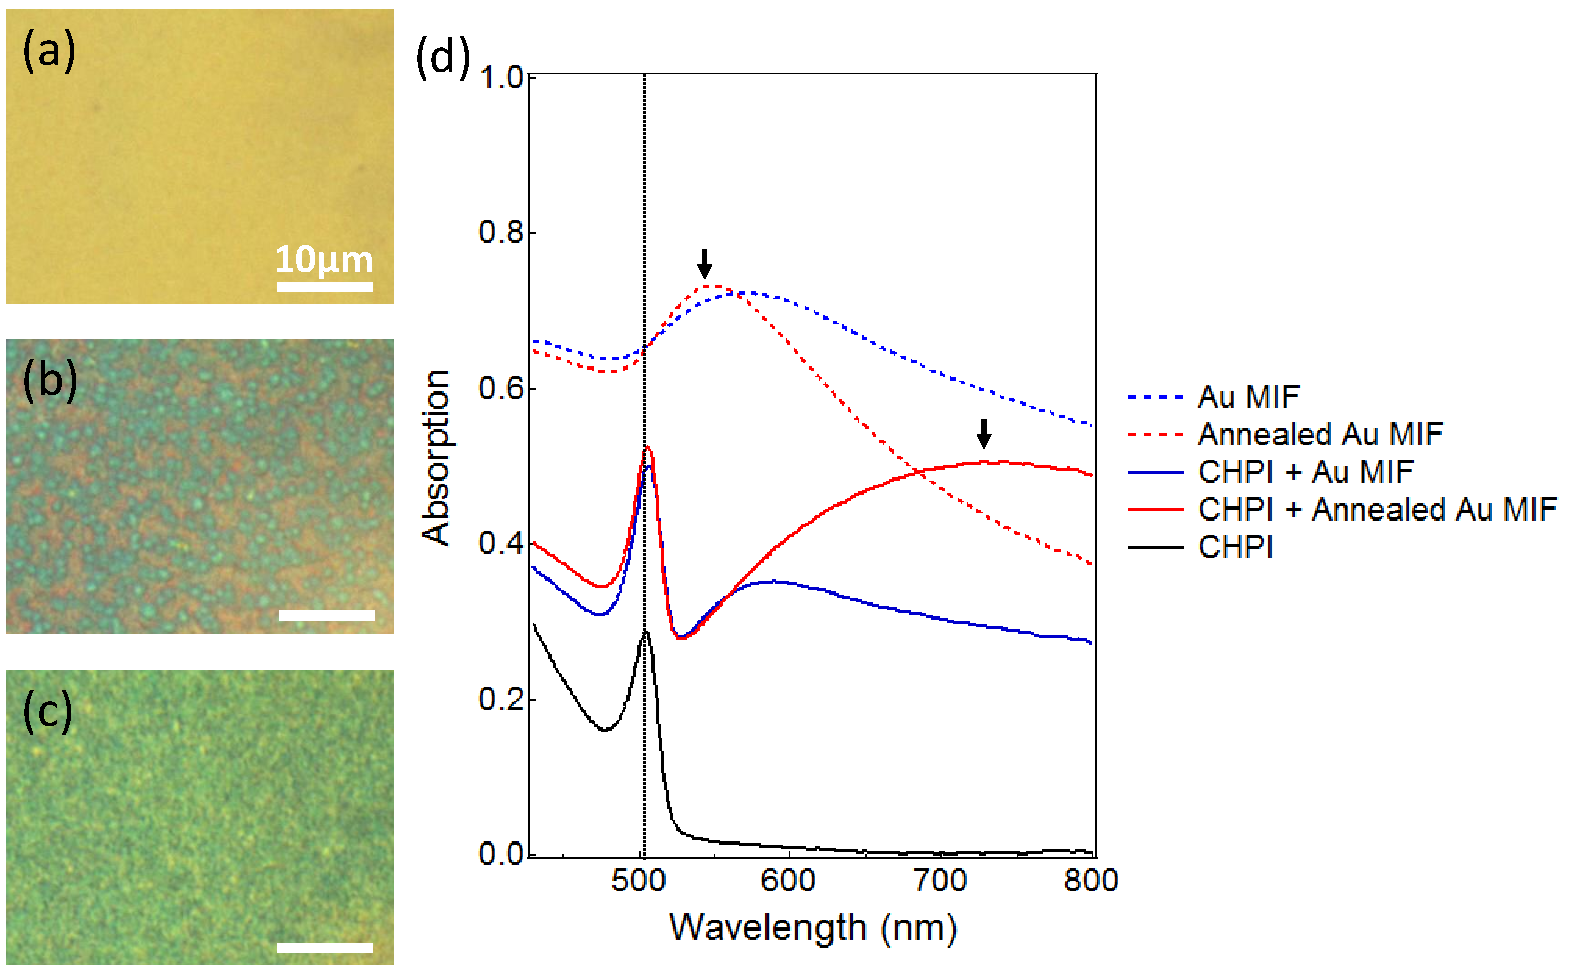
\includegraphics[width=\textwidth]{Fig3}
\caption{BF images at 100$\times$ magnification for CHPI films on (a) glass, (b) $t=8$\,nm as-deposited and (c) $t=8$\,nm annealed Au metal island films. (d) Average extinction spectra for 400 pixels over $0.5\time0.5$\,mm$^2$. The exciton wavelength is marked by the dashed line, and LSP resonances by arrows. The CHPI + (annealed) Au spectra are offset for clarity.}
\label{6Fig3}
\end{figure}
BF images at 100$\times$ magnification show the formation of CHPI on glass [Fig.\,\ref{6Fig3}(a)] and $t=8$\,nm as-deposited and annealed Au MIFs (green areas in Figs.\,\ref{6Fig3}(b,c)). The exciton resonance at 505\,nm is observed for all three films, confirming formation of the MQW structure despite some roughness and dewetting on Au substrates. We observe a redshift in the LSP resonance as a result of the CHPI coating (550\,nm to 735\,nm), with a considerable increase in the linewidth due to the non-uniform CHPI coverage (50\,nm to $\sim200$\,nm). However the excitons in CHPI are completely unaffected by the presence Au islands, remaining at the same wavelength and linewidth although the overall magnitude of the extinction across the entire visible range by around 20\%.
%CHPI+annealed Au LSP linewidth ~500nm+?

\subsection{Ag metal island films}
\begin{figure}[h!] 
\centering    
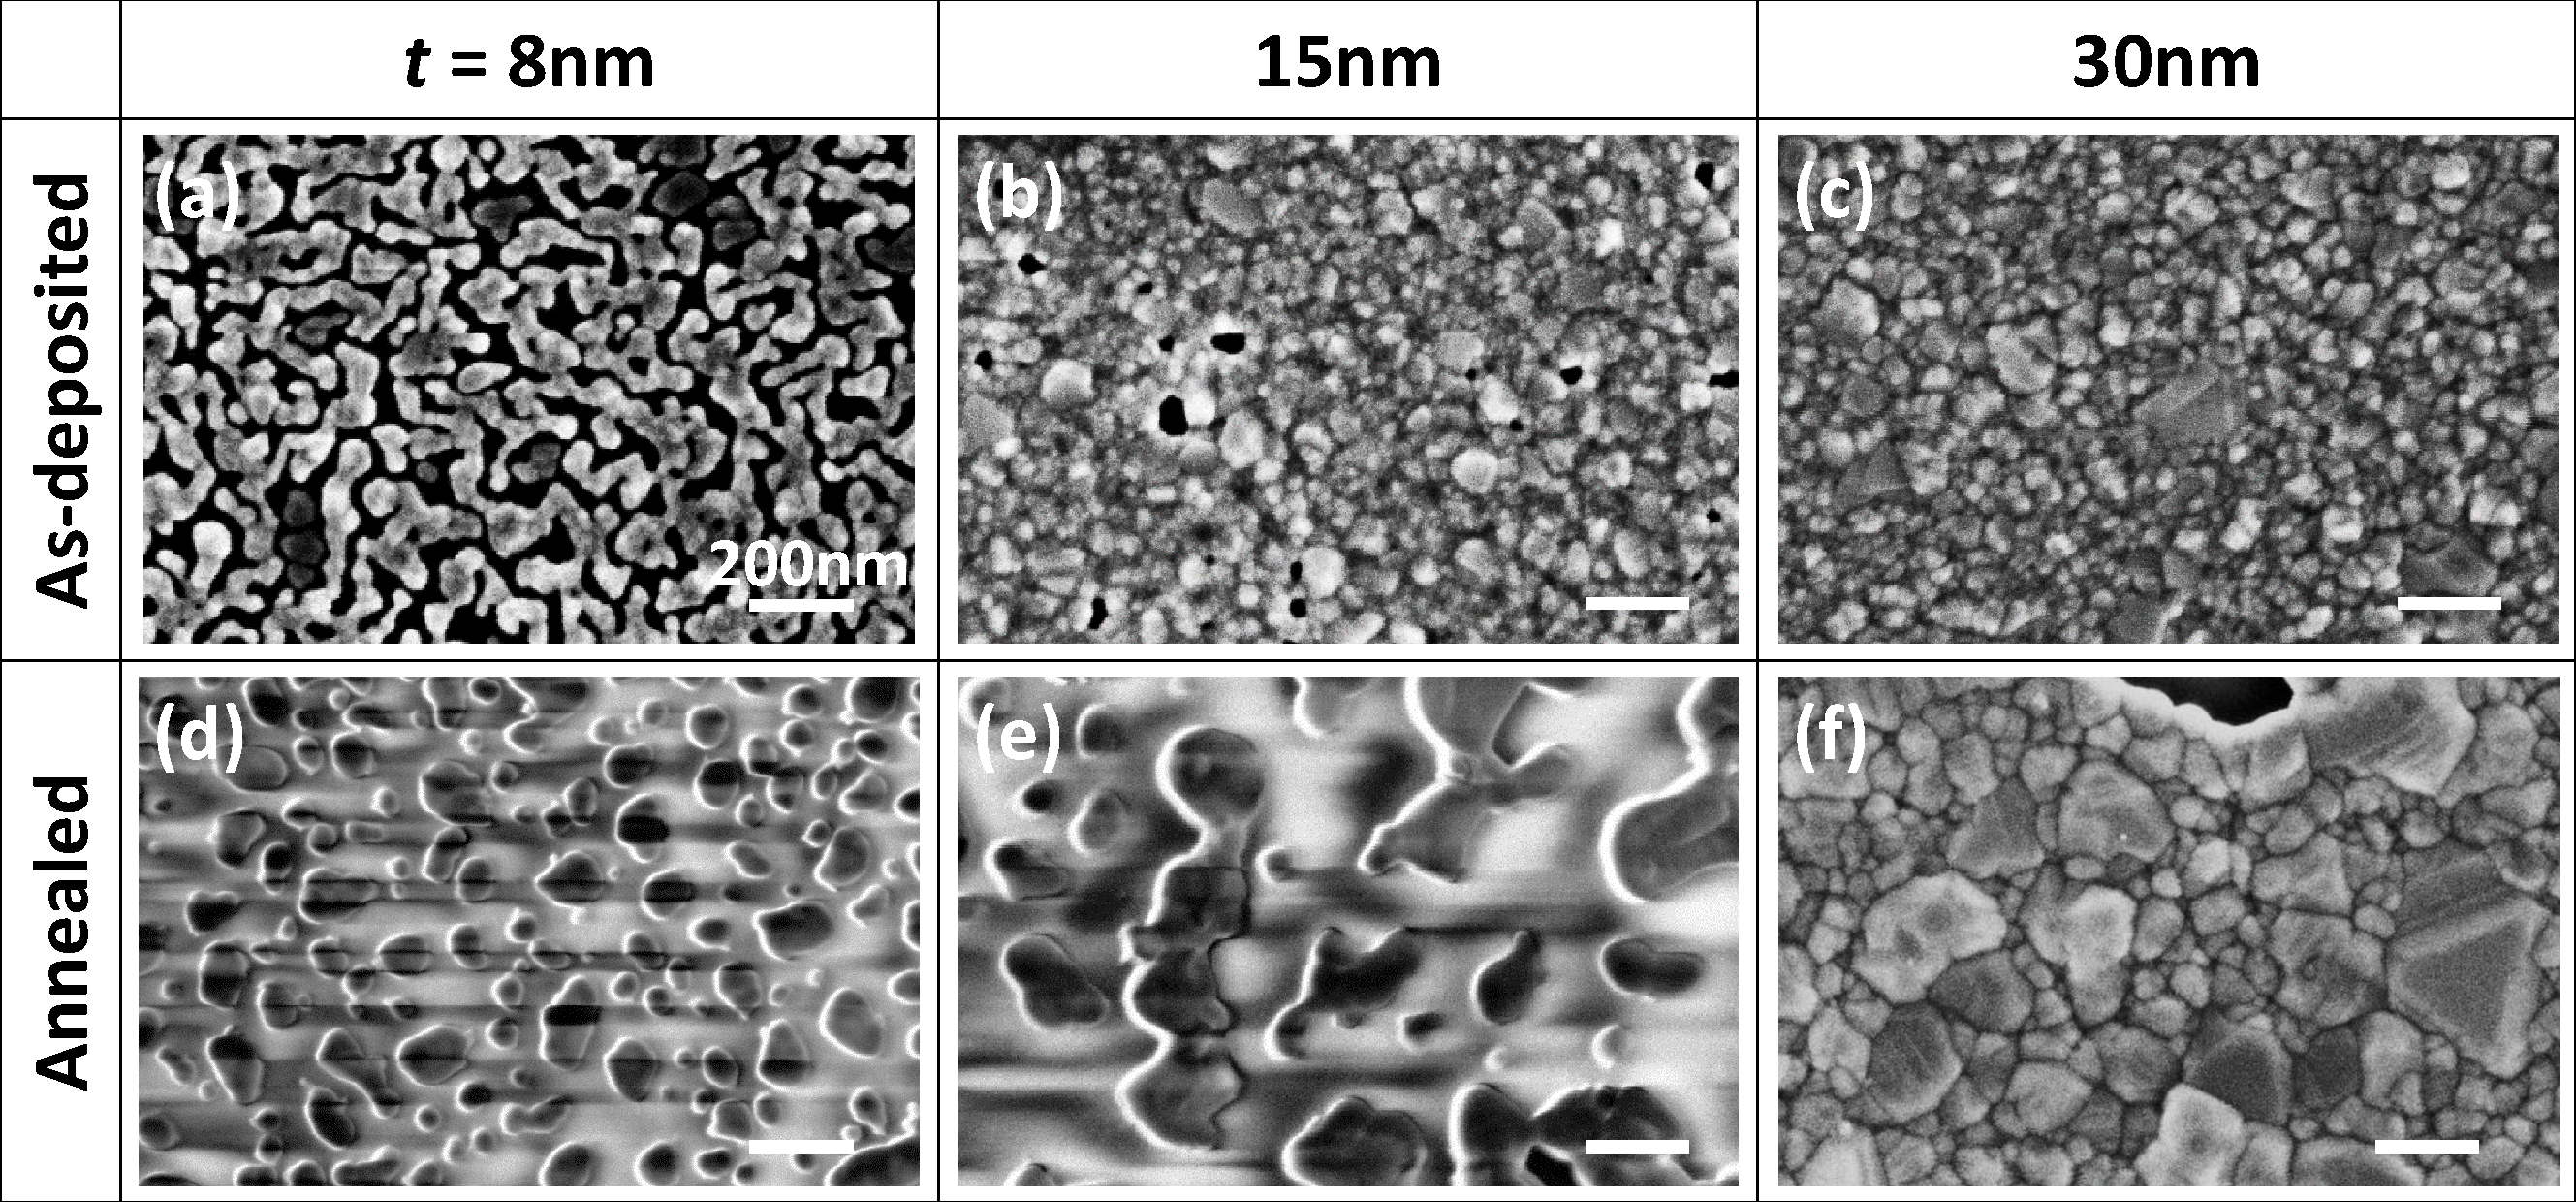
\includegraphics[width=\textwidth]{Fig4}
\caption{SEM images of (a-c) as-deposited and (d-f) annealed evaporated Ag metal island films. The initial deposited film thickness $t$ is labelled. Dark areas/streaks are seen in (a, d, e) due to charging of the sample.}
\label{6Fig4}
\end{figure}
The morphology of Ag evaporated films glass are similar to Au films: rough films lead to dewetted films with decreasing $t$, as well as formation of MIFs when the as-deposited films are annealed [Fig.\,\ref{6Fig4}]. However the interactions between Ag atoms and glass is clearly stronger as annealing only causes coalescence and larger grains for $t=30$\,nm films, not separated islands. Annealed $t=8$\,nm Ag MIFs consist of ellipsoidal islands with $d \sim40-100$\,nm, $h\sim80$\,nm, and $l\sim50-150$\,nm [Fig.\,\ref{6Fig5}]. DF images at $100\times$ magnification also show a change from broadband white scattering to green as $t$ decreases [Fig.\,\ref{6Fig5}]. 

\begin{figure}[h!] 
\centering    
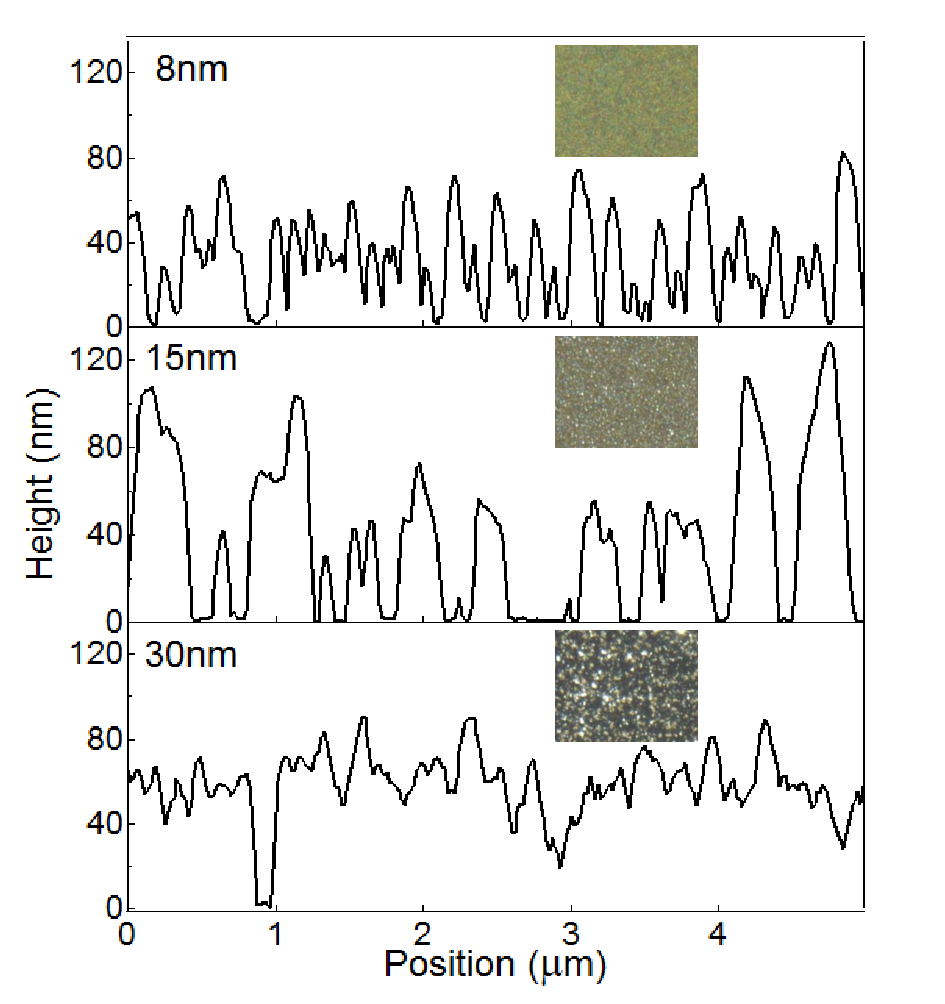
\includegraphics[width=0.8\textwidth]{Fig5}
\caption{AFM profiles of annealed Ag metal island films. The deposited film thickness $t$ is labelled. Insets show 100$\times$ magnification DF images of the samples.}
\label{6Fig5}
\end{figure}

As seen in the SEM images, as-deposited Ag films are essentially continuous with some dewetting if $t>8$\,nm. Thus extinction spectra are similar to that of bulk Ag films, with increasing extinction up to the band gap $\sim300$\,nm [Fig\,\ref{6Fig6}(a)]. However resonances can be observed if $t\leq8$\,nm, particular $t=2$\,nm (resonance 560\,nm and linewidth 175\,nm), indicating formation of islands even without annealing (Sec.\,\ref{sec:AgonCHPI}). 

After annealing, LSP resonances of Ag islands dominate the extinction spectra [Fig.\,\ref{6Fig6}(b)]. Although the positions of the extinction peaks do not change significantly with $t$, there is a clear decrease in the linewidth of the $t=2$\,nm film compared to the others [Fig.\,\ref{6Fig6}(c)]. The relative stability of the LSP wavelength suggests the average island size does not change with $t$, however we may have a larger range of island shape/size, leading to a superposition of many resonance wavelengths and higher order LSP modes. As a result of the CHPI coating the Ag island resonance is expected to redshift to $\sim550$\,nm.
\begin{figure}[h!] 
\centering    
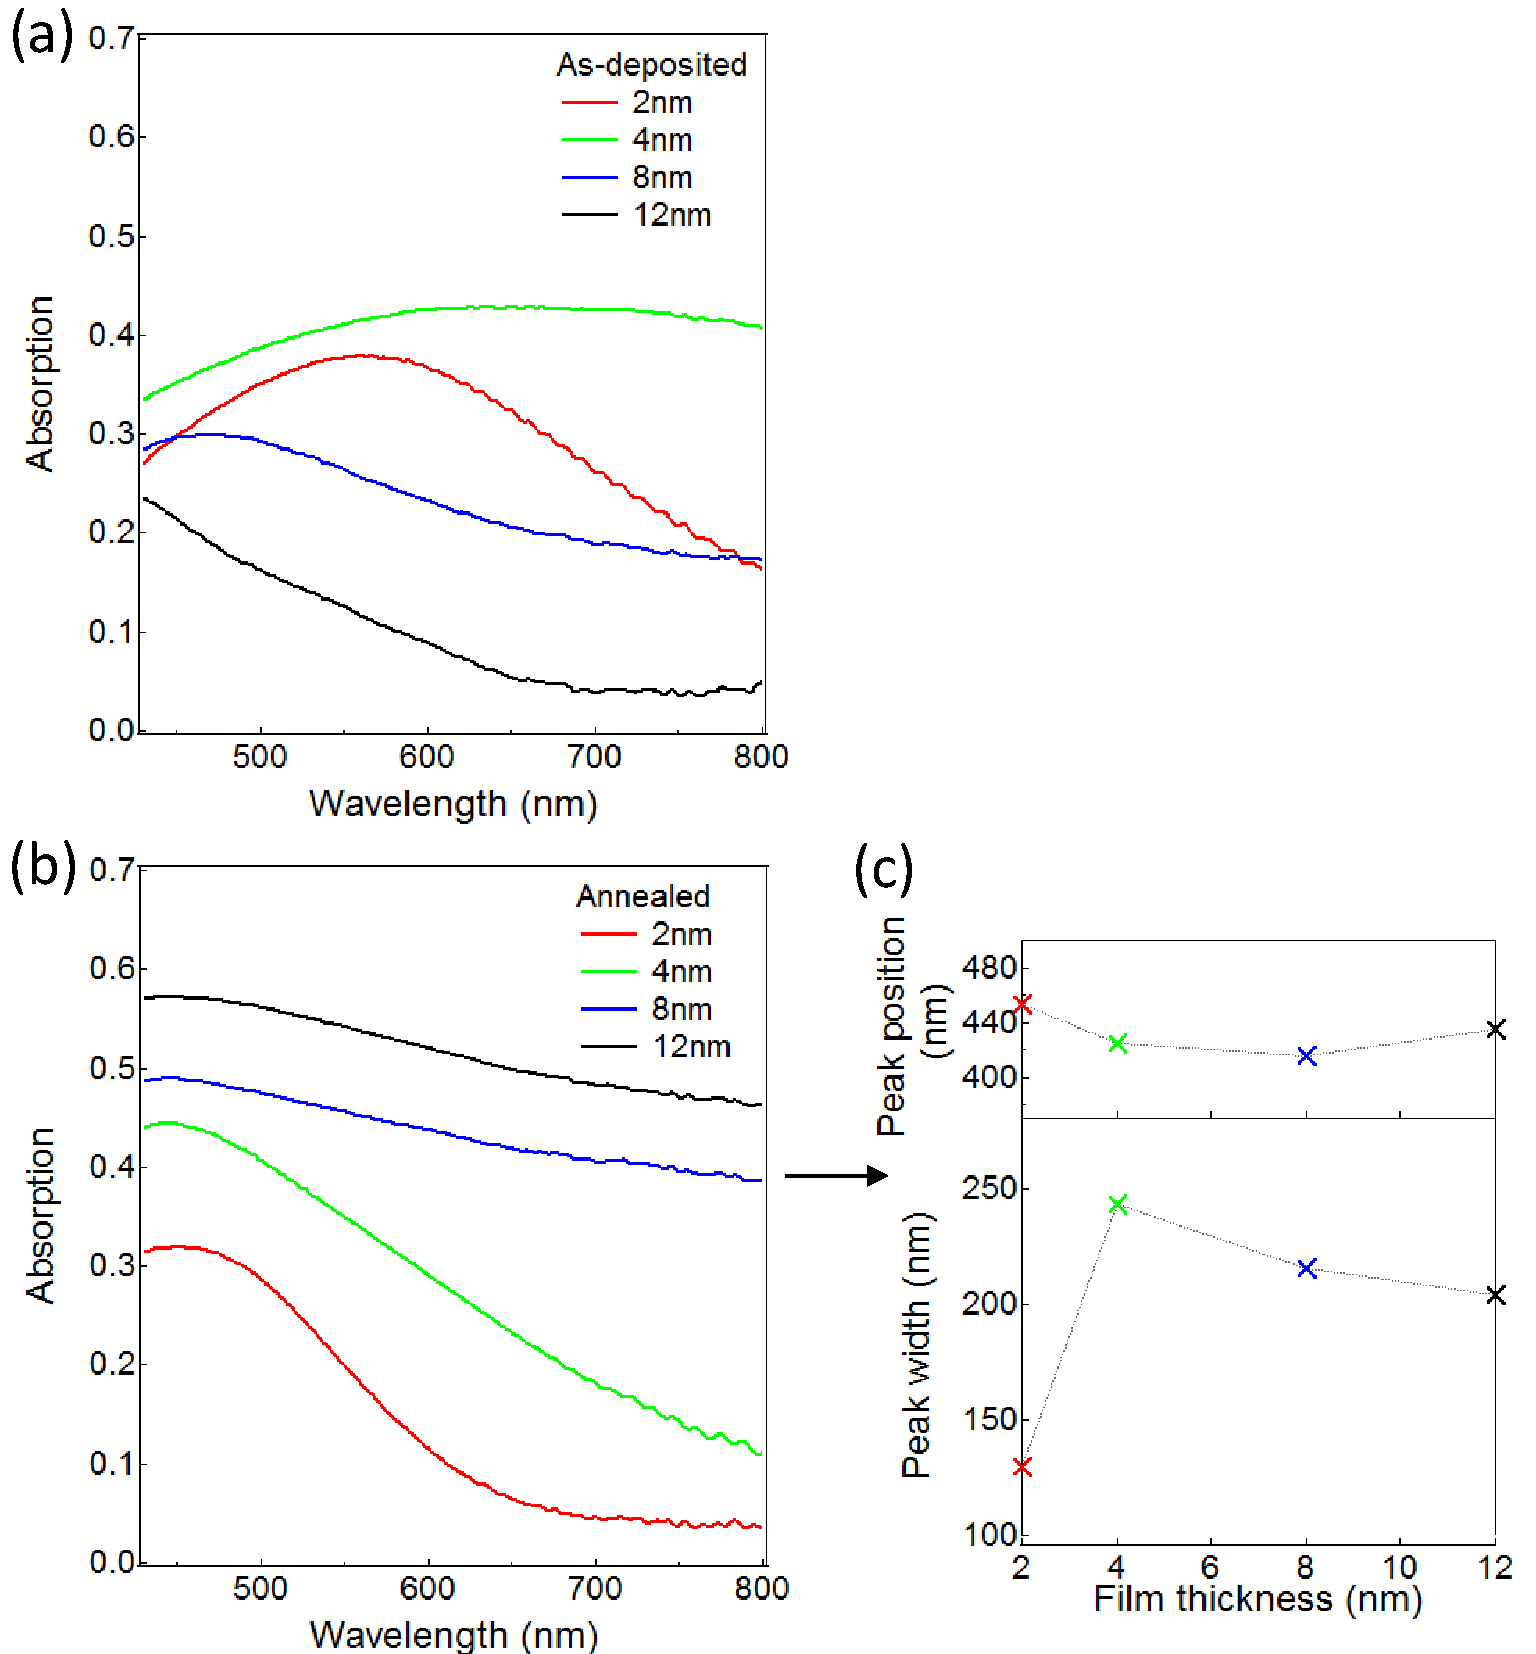
\includegraphics[width=0.8\textwidth]{Fig6}
\caption{Average extinction spectra of 400 pixels over $0.5\times0.5$mm$^2$ for (a) as-deposited and (b) annealed Ag metal island films with the labelled thickness $t$. (c) Extinction peak position and linewidth for the spectra in (b).}
\label{6Fig6}
\end{figure}

\subsection{CHPI-coated Ag metal island films}
\begin{figure}[h!] 
\centering    
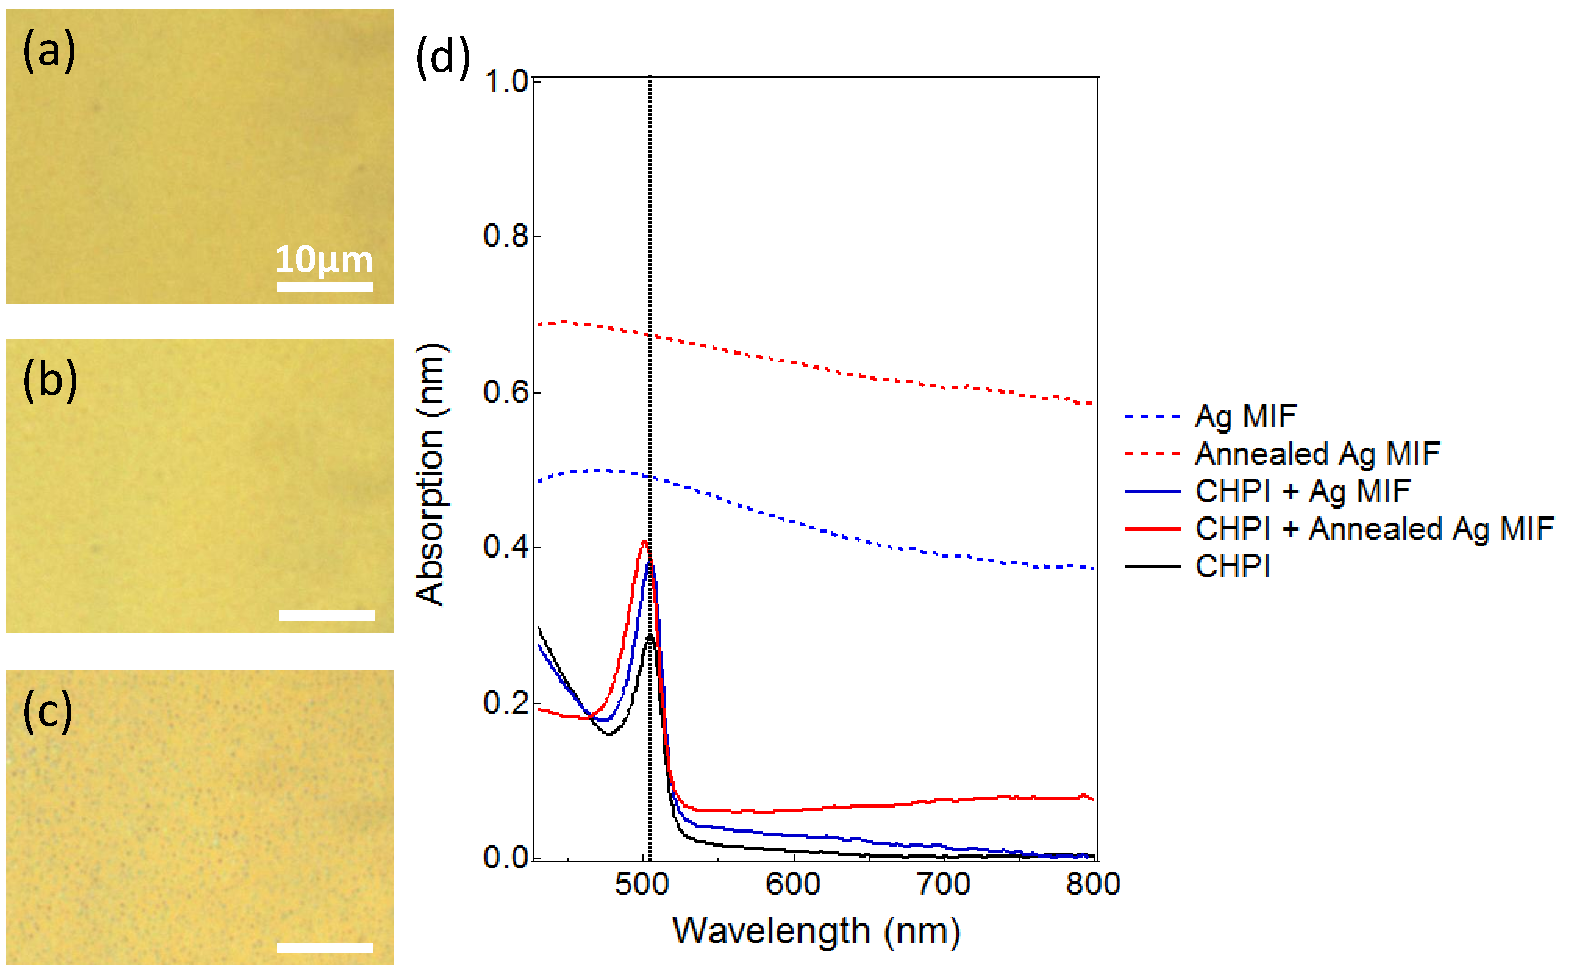
\includegraphics[width=\textwidth]{Fig7}
\caption{BF images at 100$\times$ magnification for CHPI films on (a) glass, (b) $t=8$\,nm as-deposited and (c) $t=8$\,nm annealed Ag metal island films. (d) Average extinction spectra for 400 pixels over $0.5\times0.5$mm$^2$. The exciton wavelength of the CHPI film on glass is marked by the dashed line. The (annealed) Ag MIF spectra are offset for clarity.}
\label{6Fig7}
\end{figure}
CHPI coated Ag films behave similarly for $t\leq8$\,nm, so here we use $t=8$\,nm as an example. BF images at 100$\times$ magnification show very little difference between CHPI films on glass, as-deposited or annealed Ag MIFs [Fig.\,\ref{6Fig7}(a-c)], although some non-uniformity is observed in the case of annealed Ag MIF. As-deposited Ag MIF causes little change to the exciton wavelength (505\,nm). However for annealed Ag MIF the island LSP is resonant with CHPI excitons, thus we see weak coupling in the form of a blueshift in the exciton by 5\,nm to 500\,nm, as well as an increase in the size of the exciton extinction peak by 12\%.
The extinction spectra of CHPI coated as-deposited Ag film is very similar to the spectra of CHPI film on glass (exciton at 505\,nm). However the Ag islands of the annealed film causes a blueshift of the exciton wavelength to 500\,nm, we see no appearance of the island LSP resonance, and there is an overall increase in the exciton extinction peak as a result of the Ag islands. Together this indicates weak coupling between the Ag LSP and excitons and enhancement in exciton absorption due to the near-field of the LSP. 

\subsection{Ag islands on CHPI films}
\label{sec:AgonCHPI}
\begin{figure}[h!] 
\centering    
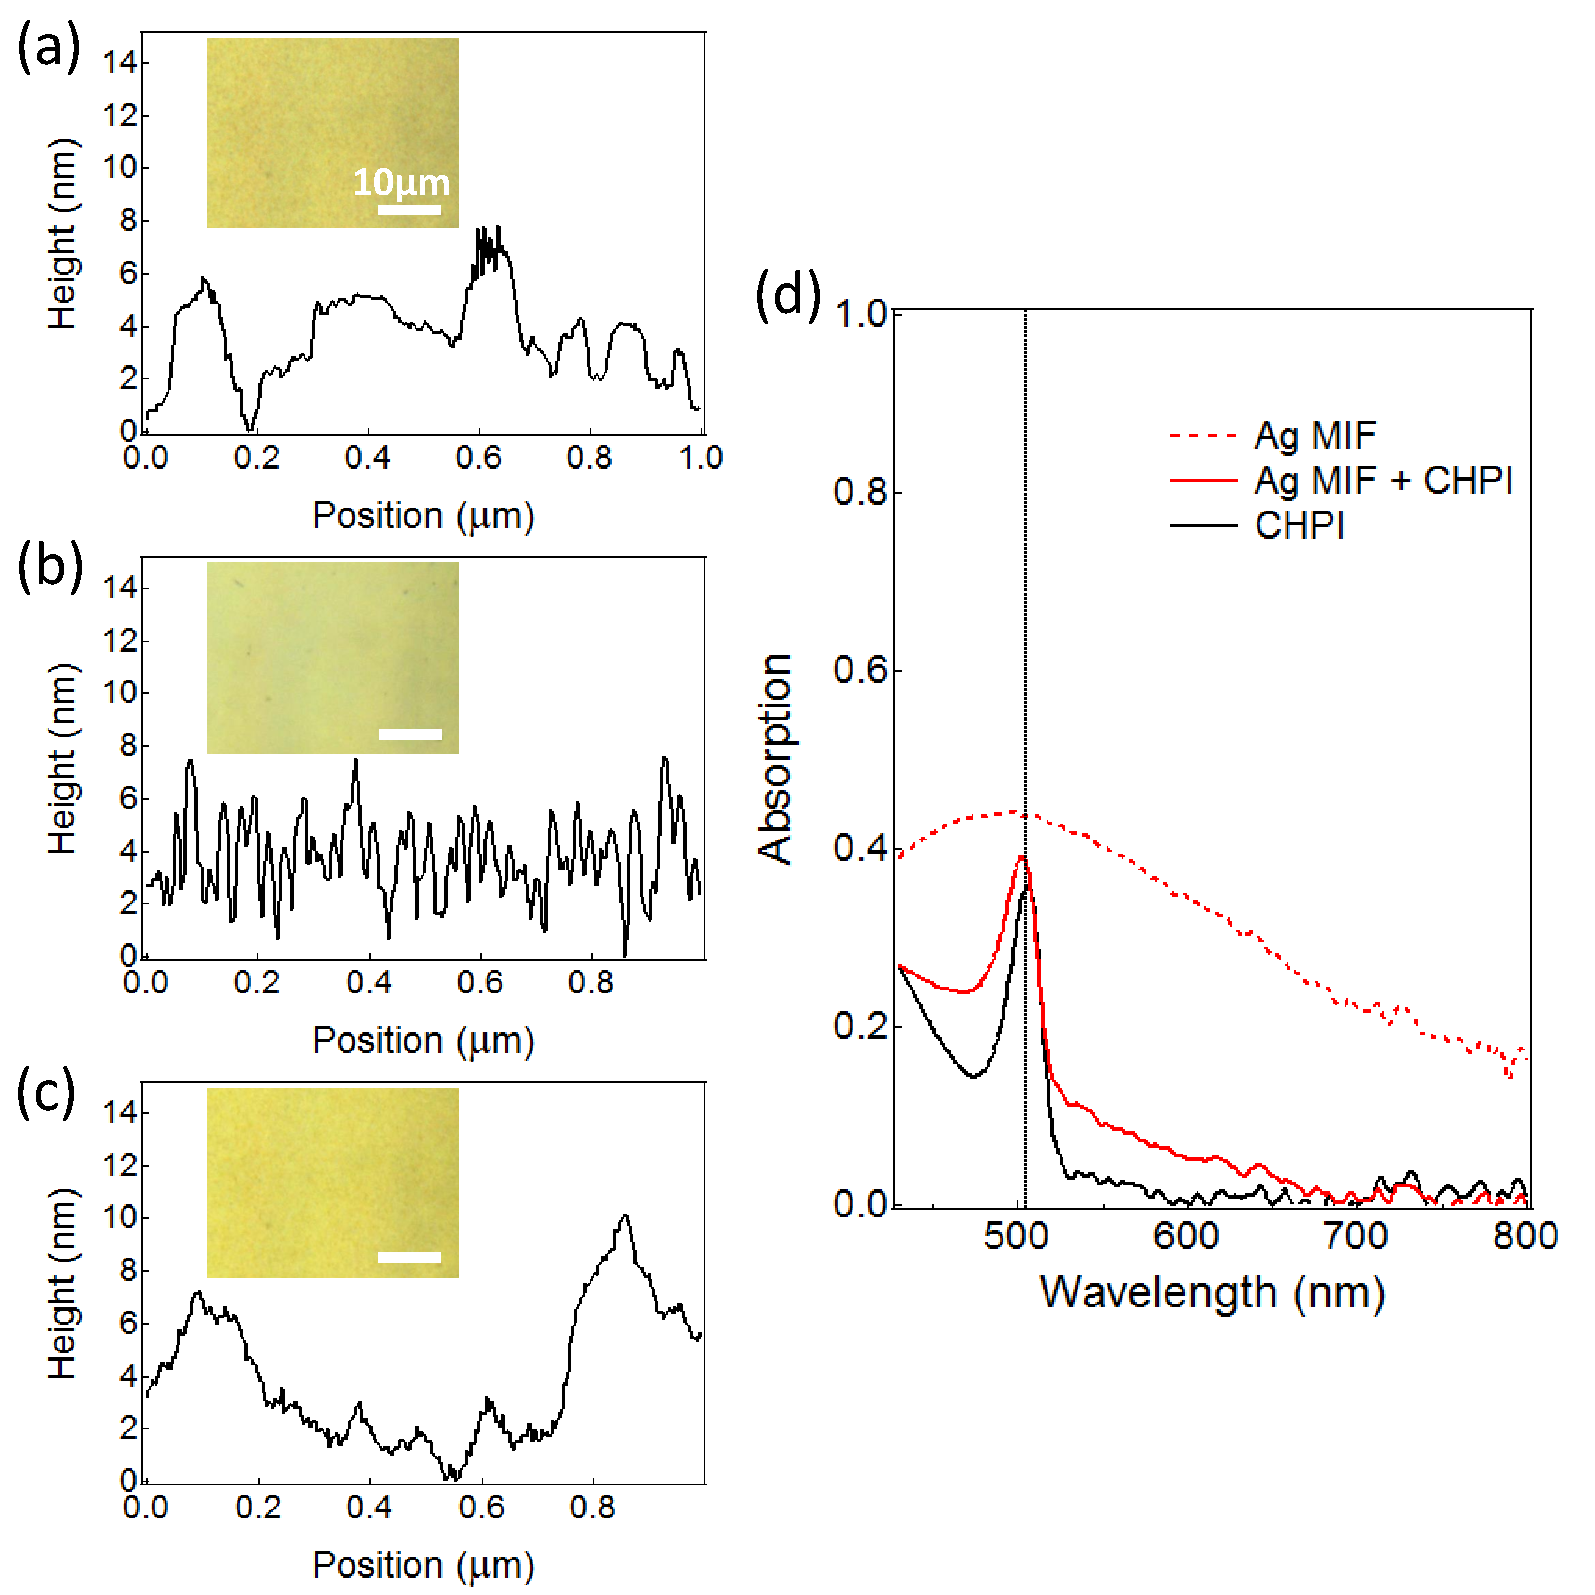
\includegraphics[width=\textwidth]{Fig8}
\caption{AFM profiles of (a) CHPI film on glass, (b) $t=2$\,nm evaporated Ag film on glass, and (c) $t=2$\,nm evaporated Ag film on CHPI. Insets show 100$\times$ magnification BF images of the samples. (d) Average extinction spectra for 400 pixels over $0.5\times0.5$mm$^2$. The exciton wavelength of the CHPI film on glass is marked by the dashed line. The Ag MIF spectrum is offset for clarity.}
\label{6Fig8}
\end{figure}
Instead of coating Ag MIF films with CHPI, we also fabricate samples of Ag islands on top of a CHPI film on glass. Since the organic molecules undergo a melting transition $\sim$80$^{\circ}$C \cite{Barman2003}, we thermally evaporate only 2\,nm of Ag to prevent degradation of the CHPI film due to heat. The AFM profile of a 2\,nm as-deposited Ag MIF on glass [Fig.\,\ref{6Fig8}(b)] shows the formation of separated metal islands, with $d\sim$30\,nm and $h\sim$6\,nm. The AFM profile of a Ag MIF on CHPI is dominated by surface roughness of the CHPI film ($\sim$5\,nm, \textit{cf} Fig.\,\ref{6Fig8}(a)), however some high frequency noise on the order of $d$ can also be seen. The lack of distinct MIF features suggests Ag islands may be partially embedded in the CHPI film. The thermal evaporation of Ag has not damaged the CHPI film as a strong exciton peak can still be seen in extinction spectra. The Ag island LSPs has again weakly coupled to excitons, causing a blueshift of 4\,nm but an increase in extinction of only 5\% [Fig.\,\ref{6Fig8}(d)].

\section{Nanosphere lithography}
Nanosphere lithography involves the evaporation of metals through a closely-packed 2D arrays of nano-/microparticles followed by removal of the spheres, leaving behind an array of metal islands on the substrate \cite{Haynes2001}. The geometry of the island array depends on the diameter of spheres $D$. For a colloidal monolayer, the island diameter is $0.223D$, while the inter-island separation is $0.58D$ \cite{Hulteen1995}. The interstices between spheres causes formation of triangular islands, however for small $D$ the islands can become more spherical \cite{Hulteen1999}. Array geometry can also be controlled by changing the evaporation angle \cite{Haynes2002}.

Much like MIFs, these triangular islands produce a LSP peak in optical spectra that depends on the size/shape of islands as well as the dielectric environment \cite{Jensen2000}, and can be modelled as an array of dipoles \cite{Malinsky2001, Jensen1999}. However nanosphere lithography provides better control of the island geometry due to the lithography mask, and should provide a sharper LSP resonance compared to MIFs.

\subsection{Experimental methods}
We use $D=460$\,nm polystyrene (PS) microspheres from Sigma Aldrich to create the colloidal monolayer. The 10\,vol\% microsphere solution in water is diluted in a 1:1 mix with ethanol (absolute). Glass substrates are cleaned as described in Sec.\,\ref{sec:glass} then plasma etched for 1\,minute to create a hydrophilic surface. The substrates are placed at a $10^{\circ}$\,angle before a deionised water droplet is applied to cover the glass surface. A 2\,wt\% solution of sodium dodecylsulphate in water ($<0.5\,\mu$l) is applied to the water surface, where the amphiphilic molecules act to reduce the surface charge on PS microspheres. A pipette is used to spread PS microspheres onto the droplet surface [Fig.\,\ref{6Fig9}(a)], and the water is allowed to evaporate under standard conditions. 50\,nm of Au is then deposited on the samples using an electron-beam evaporator system under pressure $\sim5\times10^{-6}$\,Torr at rate of 1\AA/s. The PS microspheres are dissolved by placing the sample in a solution of dichloromethane for 30\,minutes, then sonicating the solution for 5\,minutes. A CHPI/THF solution is spin coated onto the island samples under a dehydrated atmosphere. Optical characterisation is performed by taking 400 scans over a $50\times50\,\mu$m$^{2}$ region, then averaged to produce the spectra shown. 

\subsection{Au islands}
Closely-packed 2D arrays of PS microspheres are formed using this technique [Fig.\,\ref{6Fig9}(b)], and the ordering is best at contact lines. After removal of PS, triangular islands are left behind on the glass substrate [Fig.\,\ref{6Fig9}(c)] with $d\sim$90\,nm. We can see from Fig.\,\ref{6Fig9}(c) that even in the best areas we do not uniformly find well-separated triangular islands. Due to small deviations in the microsphere packing bow-tie shaped islands can form, and lines of Au are found at domain boundaries. However in the extinction spectra of such island samples [Fig.\,\ref{6Fig10}] we do observe an LSP resonance at 590\,nm with a linewidth of 80\,nm, comparable to MIF spectra.
\begin{figure}[h!] 
\centering    
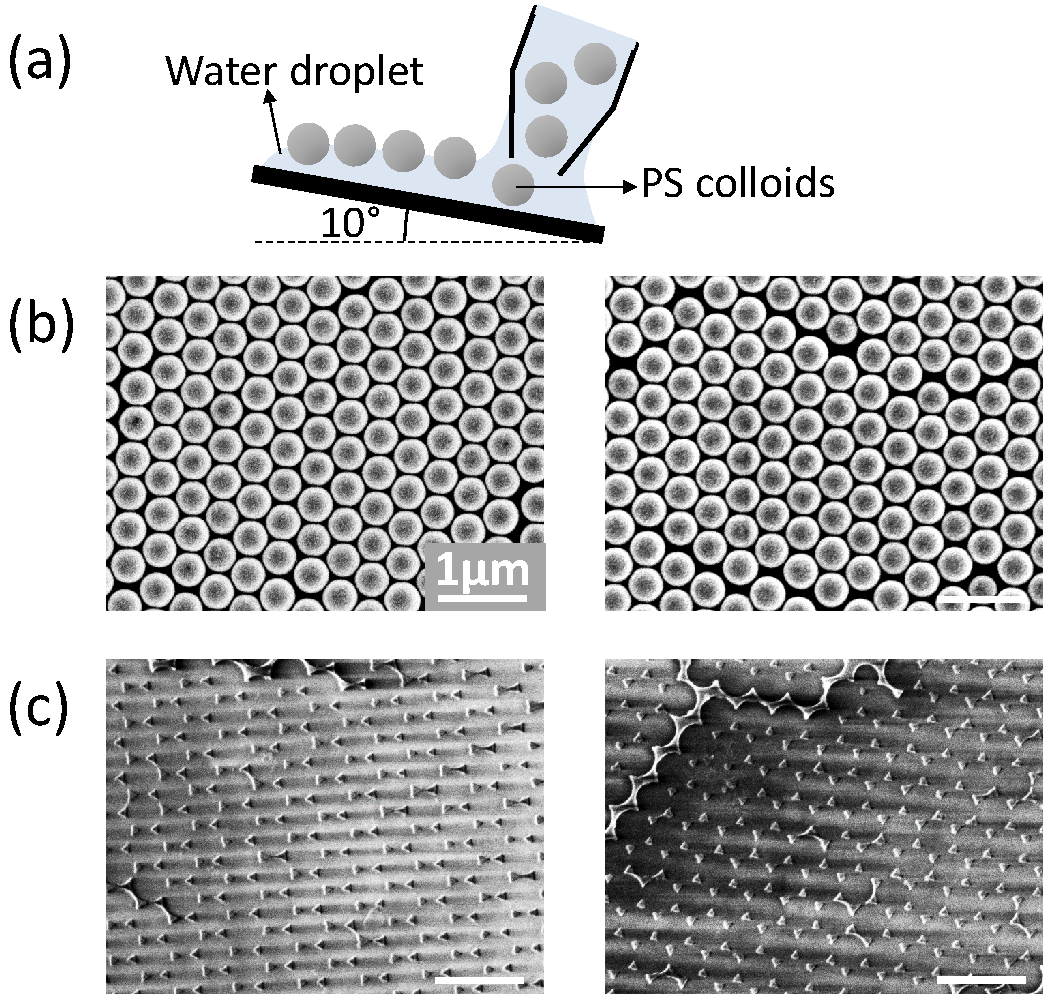
\includegraphics[width=0.8\textwidth]{Fig9}
\caption{(a) Illustration of the creation of $D=460$\,nm PS colloidal monolayer on a water droplet. (b) SEM of colloidal monolayer formed after the evaporation of water. (c) SEM of triangular islands formed after evaporation of Au and removal of colloids.}
\label{6Fig9}
\end{figure}

\subsection{CHPI-coated Au islands}
Similar to CHPI-coated Au MIFs, strong exciton peaks in the extinction spectra of CHPI-coated Au islands indicate formation of the MWQ structure. The exciton wavelength is unaffected by the Au (505\,nm). As before, the LSP resonance redshifts due to the CHPI coating, and the linewidth broadens to $\sim$150\,nm. We observe a systematic increase of the LSP redshift as a result of increasing spin speed, and attribute this to more complete CHPI encapsulation of the Au islands as a result of larger forces at high spin speeds.
\begin{figure}[h!] 
\centering    
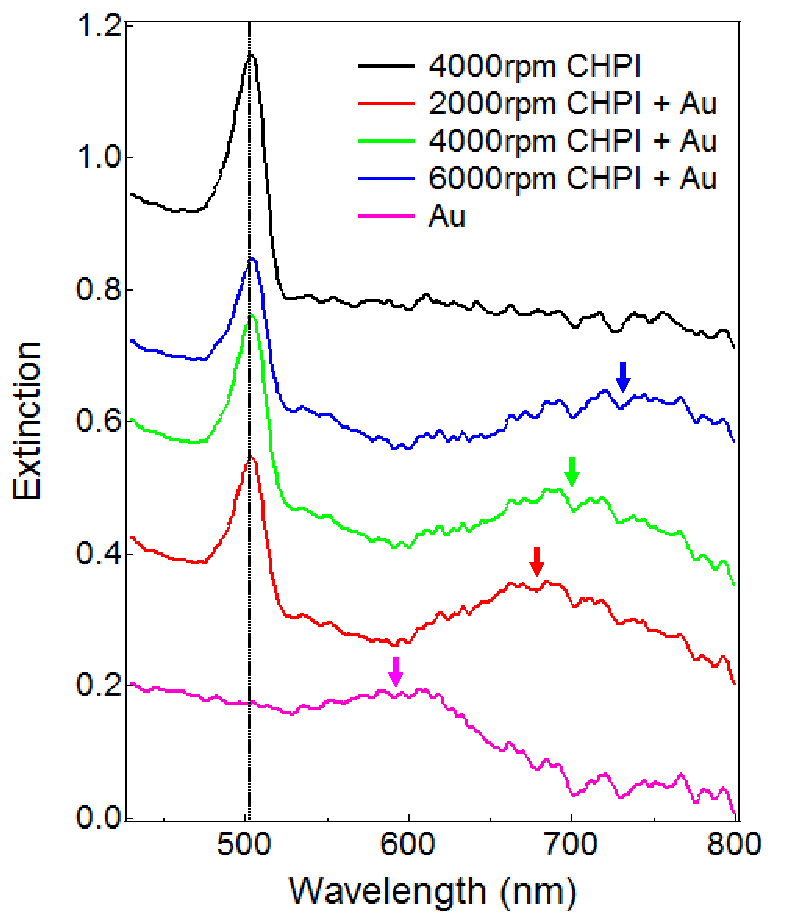
\includegraphics[width=0.8\textwidth]{Fig10}
\caption{Average extinction spectra (400 pixels over $50\times50\,\mu$m$^2$ for CHPI-coated Au islands as labelled. Arrows indicate the positions of LSP resonances, and a dashed line indicates the exciton wavelength.}
\label{6Fig10}
\end{figure}

\section{Conclusions}
Evaporation of noble metals can be use to create ellipsoidal nanoparticles on a glass substrate. These metal island films behave like a nanoparticle array, and show distinct localised surface plasmon resonances that can be tuned via deposition parameters. In the case of perovskite-coated Au islands the LSPs are far off-resonance with excitons, and the dielectric coating causes a redshift in LSPs with no effect on excitons. In the case of perovskite-coated Ag islands, LSPs weakly couple to excitons and cause a blueshift in the exciton resonance of 5\,nm, as well as an increase in exciton extinction by $\sim10$\% due to the electric field enhancement. Such enhancement has been investigated and is of particular interest for the design of solar cells \cite{Alemu2014, Zheng2011, Xu2013, Spinelli2012}.

The linewidth of the LSP resonance may be a barrier to strong coupling between plasmons and exciton in perovskite-coated nanostructures. The large variation in shape and size of metal particles in MIFs is an issue, however from our experiments more controllable islands created using nanosphere lithography do not show a marked improvement in LSP linewidth. Chemically created metallic NPs, which are often pre-screened for size, may provide an avenue for future exploration, however a method of controllably assembling a dense array of well-separated NPs from solution will need to be investigated.